\chapter{Suffix arrays}\label{ch:suffix-arrays}
Een tweede datastructuur die we in meer detail bekijken, is de suffix array.
Het voordeel van deze datastructuur is het lagere geheugengebruik in vergelijking met suffixbomen.


\section{Wat zijn suffix arrays?}\label{sec:wat-zijn-suffix-arrays?}
Suffix arrays (SAs) zijn een geheugenefficiëntere voorstelling voor de bladeren van een suffixboom.
In plaats van een boomstructuur met een veel pointers maken ze gebruik van \textbf{een array die de volgnummers van elke suffix in de originele string bevat}.
Deze volgnummers worden lexicografisch gesorteerd op basis van de overeenkomstige suffix.
Figuur~\ref{fig:suffixtree_vs_suffixarray} geeft een voorbeeld van een suffixboom en suffix array opgebouwd over de tekst \texttt{acacgt\$}.

\begin{center}
    \texttt{tekst: a|c|a|c|g|t|\$\\index: 0|1|2|3|4|5|6}
\end{center}
\begin{figure}[H]

    \begin{subfigure}[b]{0.6\linewidth}
        \resizebox{\linewidth}{!}{
            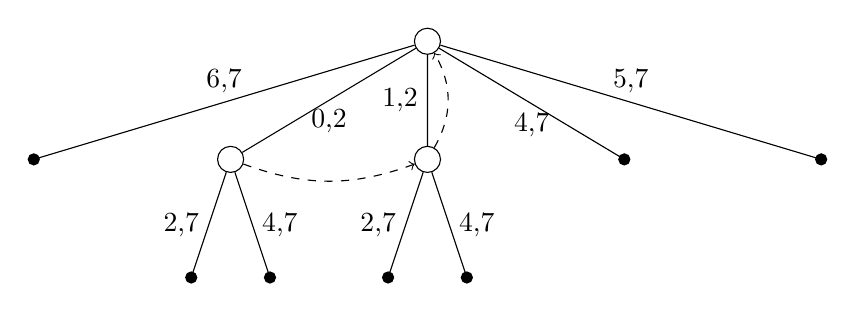
\begin{tikzpicture}
            [
                level 1/.style = {sibling distance = 2.5cm},
                level 2/.style = {sibling distance = 1cm}
            ]

                \node[draw, circle] (End2) {}
                child {
                    [fill] circle (2pt)
                    edge from parent node [above] {6,7}
                }
                child {
                    node[draw, circle] (Start1) {}
                    child {
                        [fill] circle (2pt)
                        edge from parent node [left] {2,7}
                    }
                    child {
                        [fill] circle (2pt)
                        edge from parent node [right] {4,7}
                    }
                    edge from parent node [below] {0,2}
                }
                child {
                    node[draw, circle] (End1) {}
                    child {
                        [fill] circle (2pt)
                        edge from parent node [left] {2,7}
                    }
                    child {
                        [fill] circle (2pt)
                        edge from parent node [right] {4,7}
                    }
                    edge from parent node [left] {1,2}
                }
                child {
                    [fill] circle (2pt)
                    edge from parent node [below] {4,7}
                }
                child {
                    [fill] circle (2pt)
                    edge from parent node [above] {5,7}
                }
                ;
                \draw[dashed, ->] (Start1) to[out=-20,in=200] (End1);
                \draw[dashed, ->] (End1) to[out=60,in=-60] (End2);
            \end{tikzpicture}
        }
        \caption{Suffixboom}
    \end{subfigure}
    \begin{subfigure}[b]{0.4\linewidth}
        \centering
        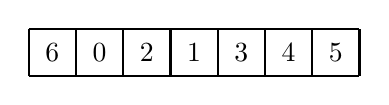
\begin{tikzpicture}[thick,scale=.6]
            \draw (0,0) grid (7,1);
            \path (.5,.5) node{$6$} foreach \i in {0,2,1,3,4,5} {++(1,0) node{$\i$}};
        \end{tikzpicture}
        \vspace{3em} % vertically center the array a bit
        \caption{Suffix array}
    \end{subfigure}

    \caption{Suffixboom en suffix array voor de string \texttt{acacgt\$}.}\label{fig:suffixtree_vs_suffixarray}
\end{figure}

Wanneer we de bladeren van de suffixboom van links naar rechts doorlopen, dan zien we dat dit overeen komt met de suffix array.
Dit is de link tussen deze twee datastructuren.
Merk op dat \textbf{de suffix array minder data bevat ten opzichte van de suffixboom}.
De interne knopen en suffix links uit de suffixboom ontbreken.
Indien deze informatie ook nodig is, kan gebruik gemaakt worden van zogenaamde Enhanced Suffix Arrays (ESAs).
Hierbij worden naast de suffix array nog drie extra tabellen bijgehouden: de Longest Common Prefix (LCP), child en suffix link tabellen.


\section{Complexiteit}\label{sec:complexiteit}
Aangezien de suffix array bestaat uit de volgnummers van de lexicografisch gesorteerde suffixen, kunnen we deze suffixen aan de hand van traditionele sorteeralgoritmen zoals merge sort~\cite{mergeSort} in $O(n^2 \log n)$ tijd en $O(n^2)$ geheugen sorteren, wat onmiddellijk de bijhorende suffix array als resultaat oplevert.
Hierbij is $n$ de lengte van de tekst.
De totale tijdscomplexiteit hiervan is $O(n^2 \log n)$ en niet $O(n \log n)$ aangezien elke vergelijking van twee suffixen in het slechtste geval $n$ karaktervergelijkingen vereist.
Ondertussen bestaan er echter verschillende algoritmen die een tijdscomplexiteit van $O(n)$ bereiken~\cite{sais, ko_alura, radixSA, dark_archon, libdivsufsort} voor het opbouwen van de suffix array van een tekst.
Bovendien vereisen deze veel minder geheugen dan een equivalente suffixboom.
Sommige implementaties vereisen slechts $5n + O(1)$ geheugen~\cite{dark_archon, libdivsufsort, libsais}.
\\ \\
Zoeken in een suffix array kan in $O(m \log n)$.
Hierbij is $n$ opnieuw de lengte van de tekst, en $m$ de lengte van de zoekstring.
Het resultaat van deze zoekopdracht is een interval in de suffix array waarbinnen de matches liggen, of een leeg interval indien er geen matches zijn.
Indien we effectief alle matches willen ophalen moeten we deze allemaal overlopen en komt de totale complexiteit uit op $O(m \log n + |Occ|)$ met $|Occ|$ het aantal gevonden matches in de tekst.


\section{Bestaande implementaties}\label{sec:bestaande-implementaties}
Aangezien er meerdere sterk geoptimaliseerde implementaties bestaan voor het opbouwen van een suffix array, vergelijken we eerst de performantie van deze implementaties.
Hieruit kunnen we nadien een snelle en geheugenefficiënte implementatie selecteren.
Tabel~\ref{tab:sa_building} bevat een overzicht van verschillende algoritmen.
Voor sommige werden verschillende implementaties getest.

\begin{table}[H]
    \begin{minipage}{\linewidth}
        \centering
        \begin{tabular}{l l S[table-format=-2.2] S[table-format=-2.2] S[table-format=-1.2] S[table-format=-1.2]}
            Algoritme & Programmeertaal & \multicolumn{2}{c}{Tijd (in s)} & \multicolumn{2}{c}{Geheugen (in GB)} \\
            \hline\hline
            &                      & {32-bit} & {64-bit} & {32-bit} & {64-bit} \\
            \cline{3-6}
            libdivsufsort\footnote{\url{https://github.com/y-256/libdivsufsort}}                                       & C                    & 15.01    & 15.97    & 1.03     & 1.86     \\
            libdivsufsort\footnote{\url{https://github.com/baku4/libdivsufsort-rs}}                                    & Rust + bindings to C & 16.00    & 15.52    & 1.03     & 1.86     \\
            libdivsufsort\footnote{\url{https://github.com/fasterthanlime/stringsearch/tree/master/crates/divsufsort}}  & Rust                 & 20.23    & {-}      & 1.03     & {-}      \\
            dark archon a4\footnote{\url{https://github.com/kvark/dark-archon}}                                        & C                    & 39.34    & {-}      & 1.09     & {-}      \\
            libsais\footnote{\url{https://github.com/IlyaGrebnov/libsais}}                                             & C                    & 6.38     & 6.46     & 1.03     & 1.86     \\
            SA-IS\footnote{\url{https://github.com/Tascate/Suffix-Arrays-in-CPP}}                                      & C++                  & 24.39    & {-}      & 3.80     & {-}      \\
            SA-IS\footnote{\url{https://github.com/sile/sais}}                                                         & C++                  & 18.73    & {-}      & 1.46     & {-}      \\
            radixSA\footnote{\url{https://github.com/mariusmni/radixSA64}}                                             & C++                  & 9.74     & 11.26    & 2.11     & 3.52     \\
            \hline
        \end{tabular}
        \caption{Uitvoeringstijd en maximaal geheugengebruik voor het opbouwen van een suffix array aan de hand van verschillende algoritmen voor de Swiss-Prot eiwitdatabank.
        Indien er een 32-bit en 64-bit integer implementatie beschikbaar was, werden deze allebei getest. Een - staat voor niet getest. Deze testen werden lokaal uitgevoerd op een M1 Pro MacBook Pro. De specificaties hiervan zijn terug te vinden in tabel~\ref{tab:macbook_hardware}.}
        \label{tab:sa_building}
    \end{minipage}
\end{table}

We kunnen concluderen dat \textbf{libsais duidelijk de snelste implementatie is om Swiss-Prot te indexeren}.
\textbf{Samen met libdivsufsort gebruikt deze de laagste hoeveelheid geheugen}, wat libdivsufsort ook interessant maakt.
Een ander voordeel dat libsais en libdivsufsort gemeen hebben, naast hun minimale geheugengebruik, is dat ze allebei een 64-bit integer implementatie hebben.
Dit is belangrijk voor het indexeren van UniprotKB omdat de totale tekst langer is dan het grootste 32-bit integer.
Dit zorgt ervoor dat alle 32-bit integer implementaties onbruikbaar zijn voor dit einddoel.
Tot slot valt ook te zien dat het verschil tussen de C en Rust versie die bindings heeft naar de C code klein is.
De overhead van het oproepen van de C code uit Rust is dus minimaal.

\subsection{Enhanced suffix arrays}\label{subsec:enhanced-suffix-arrays}
Om een indicatie te hebben van de extra hoeveelheid geheugen die nodig is om gebruik te maken van Enhanced Suffix Arrays kunnen we via de libsais bibliotheek LCP array berekenen.
Deze LCP array is slechts één van de drie extra tabellen die deel zijn van ESAs, maar het is voor ons wel de meest interessante.
De baseline waarmee we willen vergelijken is de hoeveelheid geheugen die we nodig hebben om enkel de SA op te bouwen.
Voor de Swiss-Prot eiwitdatabank was dit 2.3 GB\@.
Als we ook de LCP array berekenen, loopt het maximale geheugengebruik op naar 5.72 GB\@.
\textbf{Het berekenen van deze extra array vraagt dus ongeveer dubbel zoveel geheugen, waardoor we deze optie niet verder verkennen}.
Bovendien berekenen we deze LCP array om het voorberekenen van de geaggregeerde taxon ID voor elke interne top van de overeenkomstige suffixboom mogelijk te maken.
Daarna moet er op basis van deze SA en LCP array nog een compacte representatie gevonden worden van de boomstructuur.
Dit is niet vanzelfsprekend.


\section{Toepassen van suffix arrays op een eiwitdatabank}\label{sec:toepassen-van-suffix-arrays-op-een-eiwitdatabank}
Het moeilijkste deel van onze probleemstelling is het opbouwen van de suffix array.
Dit kunnen we oplossen aan de hand van de algoritmen uit sectie~\ref{sec:bestaande-implementaties}.
Eens we die suffix array opgebouwd hebben, blijft er echter nog een stuk van ons probleem over.
Eerst moeten we nog een mapping maken van de gevonden suffixen naar het bijbehorende eiwit.
Op basis van dit eiwit wordt daarna de LCA gezocht.

\subsection{Bouwen van de suffix array}\label{subsec:bouwen-van-de-suffix-array}
Zoals in de inleiding van sectie~\ref{sec:probleemstelling} beschreven wordt, willen we Rust gebruiken vanwege de combinatie tussen \textit{memory safety} en hoge performantie.
We willen echter gebruikmaken van de al bestaande geoptimaliseerde algoritmen om een suffix array op te bouwen.
Om beide doelen te bereiken, maken we gebruik van de interoperabiliteit tussen Rust en C/C++.
Zo bestaan er al bindings\footnote{\url{https://crates.io/crates/libdivsufsort-rs}} van Rust naar de originele implementatie van libdivsufsort\cite{libdivsufsort} (in C).
Ook al blijkt uit het testen dat dit algoritme voor het opbouwen van de indexstructuur over een kleinere eiwitdatabank niet het snelste is, is het geheugengebruik wel minimaal.
Dit laat toe om te experimenteren met het opbouwen van een SA zonder al te veel extra werk, en al onmiddellijk te zien hoe het geheugengebruik evolueert.
\\ \\
Later hebben we zelf nog een simple Rust wrapper geschreven rond de libsais C-code.
Hiervoor hebben we de \texttt{bindgen}\footnote{\url{https://crates.io/crates/bindgen}} crate gebruikt.
Op deze manier was het ook mogelijk om gebruik te maken van de snellere libsais algoritme eens we wisten dat SAs een efficiënte en schaalbare oplossing waren voor de probleemstelling.
\\ \\
Het nadeel van het gebruiken van deze bindings naar C-code is dat het oproepen van de effectieve C-code gebeurt in een \texttt{unsafe} blok.
Hierbij is het dus mogelijk dat er geheugenfouten in het programma sluipen.
Dit risico is echter miniem aangezien dit bestaande, geteste bibliotheken zijn.
Bovendien zijn we ook zeker dat eventuele geheugenfouten enkel hierdoor kunnen ontstaan en is dit de verantwoordelijkheid van de ontwikkelaar van de bibliotheek.
Dit is dus een afweging tussen optimale performantie (waarbij we het wiel niet hoeven heruit te vinden), en garantie van \textit{memory safety}.

\subsection{Mapping van suffix naar proteïne}\label{subsec:mapping-van-suffix-naar-proteine}
Bepalen welke proteïne hoort bij een bepaalde suffix kan op twee manieren.
\textbf{Een eerste optie, laten we deze een \textit{dense mapping} noemen, is om expliciet voor elke suffix bij te houden bij welke proteïne die hoort}.
Dit kan aan de hand van een array die even lang is als het aantal suffixen.
Het voordeel van deze aanpak is dat het vinden van de bijbehorende proteïne in $O(1)$ tijd kan, hiervoor is echter wel $O(m)$ geheugen nodig, met $m$ de lengte van de totale tekst.
\\ \\
\textbf{De tweede optie, aan de hand van een \textit{sparse mapping}, is om enkel de eerste of laatste suffix per proteïne bij te houden}.
Het voordeel van deze aanpak is dat er minder geheugen nodig is, meer precies $O(p)$ geheugen met $p$ het aantal proteïnen.
Het nadeel is dan weer dat het vinden van de bijbehorende proteïne trager is.
Dit neemt $O(\log p)$ tijd in beslag aan de hand van binair zoeken.
\\ \\
In Figuur~\ref{fig:dense_vs_sparse} wordt de uitvoeringstijd voor beide implementaties vergeleken.
\textbf{Standaard (en in alle komende testen) zullen wij gebruikmaken van de \textit{sparse mapping} aangezien de performantie impact in de praktijk beperkt is, en er een significante hoeveelheid geheugengebruik uitgespaard kan worden}.
Zo loopt het verschil in geheugengebruik op tot 0.8 GB voor Swiss-Prot.
Dit is maar liefst 25\% van de indexgrootte bij de \textit{dense mapping}.
Het grote verschil in uitvoeringstijd bij het Human-Prot peptidebestand valt te verklaren vanwege het extreem hoog aantal matches dat daar te vinden is voor de korte peptiden.
In de praktijk zullen we dit maximaal aantal matches echter limiteren (zie sectie~\ref{subsec:zoeken}).
Dit zal op zijn beurt ook de overhead van de sparse mapping beperkt houden.
\begin{figure}[H]
    \centering
    \subfloat[Tijd nodig om alle matches te zoeken.]{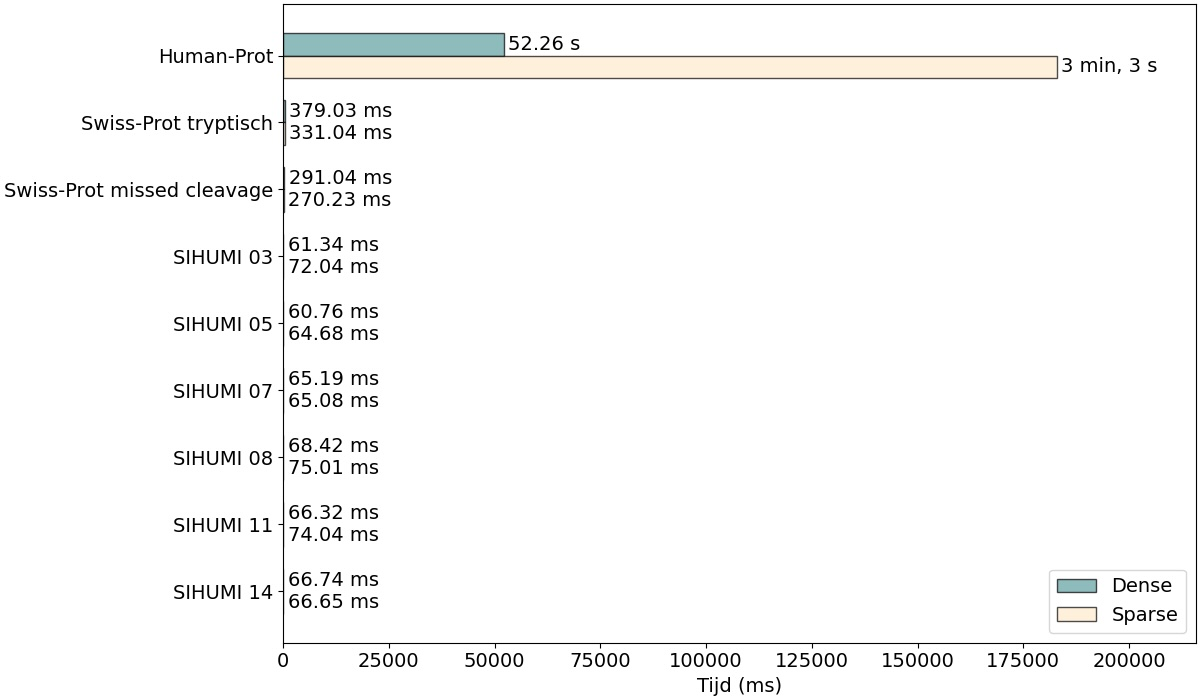
\includegraphics[width=\linewidth]{dense_vs_sparse_time}}\\[4ex] % [4ex] om wat extra vertical spacing in te voegen

    \subfloat[Maximaal gebruikt geheugen tijdens het zoeken naar alle matches.]{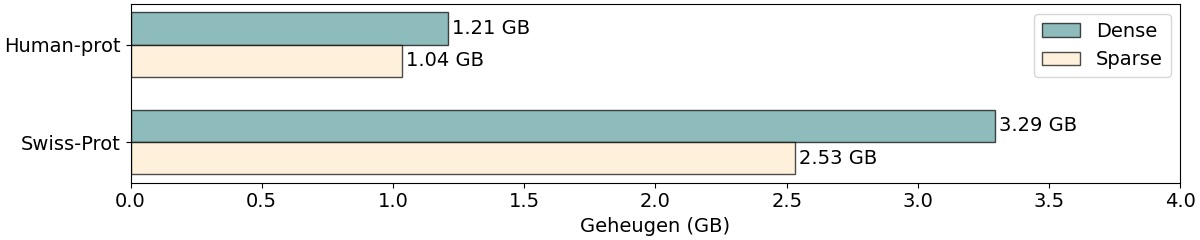
\includegraphics[width=\linewidth]{dense_vs_sparse_memory}}
    \caption{Zoektijd en geheugengebruik bij het gebruik bij een \textit{dense} of \textit{sparse mapping} van de suffixen naar de proteïnes.}\label{fig:dense_vs_sparse}
\end{figure}

\subsection{Berekenen van de LCA}\label{subsec:berekenen-van-de-lca}
Zoals eerder vermeld, bevat een suffix array geen informatie over de interne toppen die voorkomen bij een suffixboom.
Dit zorgt ervoor dat het niet mogelijk is om op basis hiervan de LCA van de organismen voor te berekenen voor al deze interne toppen.
Dit moet nu \textit{on the fly} gebeuren tijdens het zoekproces zelf.
Hierdoor is er ook \textbf{geen reden meer om LCA te gebruiken in de plaats van LCA*}.
LCA* was namelijk onze eerste keuze aangezien het resultaat hierbij minder onderhevig is aan eiwitten die een te algemene annotatie hebben.
Bij suffixbomen zijn we daar echter van af moeten stappen om het voorberekenen efficiënter te maken.


\section{Sparse en compressed suffix arrays}\label{sec:sparse-en-compressed-suffix-arrays}
Om het geheugengebruik van suffix arrays verder te verkleinen, kan er gebruikgemaakt worden van sparse of compressed suffix arrays.
In principe doen ze allebei hetzelfde.
Er wordt namelijk slechts een stuk van de originele suffix array bijgehouden.
Het verschil zit in welk stuk bijgehouden wordt.
Zoals het gezegde \textit{There is not such thing as free lunch} ons vertelt, heeft alles zijn voor- en nadelen.
Het verkleinen van de SA heeft een negatieve impact op de zoekperformantie.
We zullen namelijk slechts een deel van de peptide kunnen zoeken in de verkleinde SA\@.
Dit deel van de peptide is natuurlijk korter dan de volledige peptide, en zal in het algemeen meer matches opleveren.
Daarna moet voor elk van deze matches het niet-gematchte deel van de peptide nog gecontroleerd worden.
\\ \\
\textbf{Sparse suffix arrays (SSAs)} bouwen een suffix array op basis van elke k-de suffix van de input tekst.
Indien we slechts 50\% van de suffixen bijhouden, komt dit erop neer dat enkel suffixen die beginnen op een \textbf{even index in de inputtekst} bijgehouden worden.
Bij \textbf{compressed suffix arrays (CSAs)} wordt daarentegen slechts elke k-de waarde van de SA bijgehouden.
Indien we in dit geval 50\% van de suffixen bijhouden komt dit erop neer dat enkel suffixen die op een \textbf{even index staan in de opgebouwde suffix array} over blijven.
\\ \\
Voor beide opties is de populairste manier om ze op te bouwen aan de hand van \textbf{\textit{sampling} op de volledige SA\@}.
Hierdoor blijft het maximale geheugengebruik tijdens het opbouwen identiek aan het gebruik van de volledige SA\@.
De resulterende index zal wel kleiner zijn, waardoor de server die deze index zal hosten lagere geheugenvereisten heeft.
\\ \\
Het samplen van een opgebouwde suffix array is de meest gebruikte methode tot op vandaag, vanwege de bestaande sterk geoptimaliseerde implementaties van de klassieke SA constructiealgoritmen.
Bij sparse suffix arrays is het beste algoritme qua tijdscomplexiteit tot nu toe een Monte Carlo algoritme dat $O(n)$ tijd en $O(b)$ geheugen nodig heeft en een Las Vegas algoritme dat $O(n \sqrt{\log b})$ tijd en $O(b)$ geheugen verbruikt.
Hierbij is $n$ de lengte van de tekst, en $b$ het aantal effectief gebruikte suffixen in de sparse SA~\cite{building_sparse_sa}.
Van het Monte-Carlo algoritme is er een bestaande implementatie\footnote{\url{https://github.com/lorrainea/SSA/tree/main/MA}}.
Wanneer we aan de hand hiervan een SSA met sparseness factor 3 voor Swiss-Prot opbouwen, blijkt dit niet alleen trager te zijn ($\pm$ 10 minuten).
Ook het geheugengebruik ligt merkelijk hoger ($\pm$ 10 GB).
Terwijl we slechts een tiental seconden nodig hebben om de standaard SA op te bouwen in combinatie met 1.8 GB RAM\@.
Voor compressed suffix arrays bestaat er een algoritme dat een tijdscomplexiteit van $O(n)$ heeft in combinatie met $O(n \log \sigma)$ bits aan geheugen~\cite{building_compressed_sa}.
Hierbij is $n$ de tekstlengte en $\sigma$ de alfabetgrootte.
\\ \\
Het grootste nadeel aan deze algoritmen in de context van deze thesis is dat er nog geen sterk geoptimaliseerde implementaties bestaan.
Bovendien zal de \textbf{factor van ingevoegde sparseness in ons geval altijd vrij klein} zijn om de zoektijden beperkt te houden (aangezien we werken met een erg grote dataset en vrij korte strings).
Indien we dus een implementatie hebben om rechtstreeks een CSA of SSA te bouwen, maar met een grotere constante qua geheugengebruik, zal vanwege de kleine sparseness factor de winst snel verloren gaan.
\textbf{In ons geval is een SSA interessanter dan een CSA} omwille van de verschillende restricties tijdens het zoeken die een SSA en CSA hebben.
\\ \\
Bij het gebruik van sampling factor $k$ kunnen we bij een SSA alle sequenties van lengte $k$ en groter zoeken.
Bij een CSA is het mogelijk dat ook sommige sequenties die groter zijn dan $k$ niet te vinden zijn, en sommige kortere wel.
Dit omdat het mogelijk is dat er in het slechtste geval een gat van $n - \frac{n}{k}$ suffixen zit tussen twee opeenvolgende bijgehouden suffixen in de CSA\@.
Hierbij is $n$ de lengte van de invoertekst.
Het zoeken van extreem korte sequenties is echter niet interessant omdat deze erg weinig informatie bevatten, terwijl het verliezen van enkele langere sequenties (zonder te kunnen voorspellen welke) net extra informatieverlies met zich meebrengt.
\\ \\
Bovenstaand probleem kan opgelost worden door gebruik te maken van extra datastructuren.
Zo kan een FM-index~\cite{fm_index} gebruikmaken van een CSA, en kunnen we hierbij wel alle sequenties zoeken.
Om dit te doen moeten we echter tijdens het opbouwen van de indexstructuur nog bijkomende onderdelen berekenen (zoals de BWT\footnote{Burrows–Wheeler transformatie~\cite{bwt}} van de tekst).
Dit verhoogt opnieuw het geheugengebruik en de uitvoeringstijd tijdens het opbouwen.

\subsection{Zoeken met sparse suffix arrays}\label{subsec:zoeken-in-sparse-suffix-arrays}
Het zoeken met een SSA is erg gelijkaardig aan het zoeken met een volledige SA\@.
Een belangrijke \textbf{restrictie} is echter dat met de SSA \textbf{geen strings gezocht kunnen worden die kleiner zijn dan de sparseness factor $k$}.
Bovendien heeft deze sparseness factor ook impact op de zoekperformantie.
Bij het zoeken met sparseness factor $k$ moeten we $k$ verschillende zoekopdrachten uitvoeren.
In zoekopdracht $i$ worden de eerste $i - 1$ tekens van de zoekstring overgeslagen.
In plaats van de zoekstring, zoeken we dus een suffix van de zoekstring in de sparse indexstructuur.
\\ \\
Voor elke matchende suffix (stel dat dit suffix $s$ is) moet daarna gecontroleerd worden of de overgeslagen prefix van $i$ tekens matcht met de $i$ tekens die op posities $[s - i, i[$ in de geïndexeerde tekst staan.
Naast de SSA moet dus ook de volledige tekst in het werkgeheugen bijgehouden om te zoeken in de (sparse) SA\@.
Als dit zo is, dan matcht suffix $s - i$ met de gezochte string.
Het eindresultaat is de unie van de resultaten van elke iteratie.
Figuur~\ref{fig:sparse_sa} geeft een voorbeeld van het opzoeken van de peptide \texttt{acg} in de tekst \texttt{acacgt\$}.
Hierbij wordt gebruikgemaakt van een SA met sparseness factor $k$ = 3.

\begin{center}
    \texttt{tekst: a|c|a|c|g|t|\$\\index: 0|\textcolor{lightgrey}{1}|\textcolor{lightgrey}{2}|3|\textcolor{lightgrey}{4}|\textcolor{lightgrey}{5}|6}
\end{center}
\begin{figure}[H]
    \hfill
    \begin{subfigure}[t]{0.45\linewidth}
        \centering
        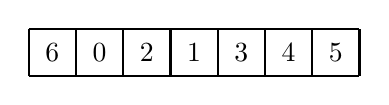
\begin{tikzpicture}[thick,scale=.6]
            \draw (0,0) grid (7,1);
            \path (.5,.5) node{$6$} foreach \i in {0,2,1,3,4,5} {++(1,0) node{$\i$}};
        \end{tikzpicture}
        \caption{Suffix array}
    \end{subfigure}
    \hfill
    \begin{subfigure}[t]{0.45\linewidth}
        \centering
        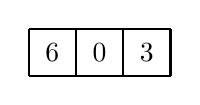
\begin{tikzpicture}[thick,scale=.6]
            \draw (0,0) grid (3,1);
            \path (.5,.5) node{$6$} foreach \i in {0,3} {++(1,0) node{$\i$}};
        \end{tikzpicture}
        \caption{Sparse suffix array met sparseness factor 3.}
    \end{subfigure}
    \hfill
    \caption{SA en SSA voor de tekst \texttt{acacgt\$}.}
    \label{fig:sparse_sa}
\end{figure}

\begin{enumerate}
    \item Sla 0 tekens over.
    Zoek \texttt{acg} met de SSA\@.
    We vinden geen matches.
    \item Sla 1 teken over.
    Dit wil zeggen dat we \texttt{cg} zoeken met de SSA\@.
    Dit levert één match op met suffix 3 (op index 1 in de SSA).
    \begin{enumerate}
        \item Controleer of de suffix die deels gematcht is ook volledig matcht met onze zoekstring.
        Dit wil zeggen dat we de overgeslagen prefix van $i = 1$ tekens (in dit geval de letter \texttt{a}) moeten kunnen matchen met de eerste $i$ tekens van suffix $3 - 1 = 2$.
        \item We zien dat het eerste teken van suffix 2 inderdaad een \texttt{a} is.
        Dit kan rechtstreeks via de tekst gecontroleerd worden aan de hand van $i$ karakters die vergeleken moeten worden.
        Suffix 2 is dus een match voor de zoekstring \texttt{acg}.
    \end{enumerate}
    \item Sla 2 tekens over.
    Zoek \texttt{g} in de SSA\@.
    We vinden geen matches.
    \item We concluderen dat enkel suffix 2 matcht met de gezochte string \texttt{acg}.
\end{enumerate}

\subsubsection{Performantie en indexgrootte}
Aangezien de sparseness factor $k$ impact heeft op de zoekperformantie is het belangrijk te zien hoe groot deze impact is, zodat we een goede keuze kunnen maken.
Op het eerste gezicht lijkt het vergroten van deze factor enkel meer iteraties toe te voegen, maar dit heeft zware gevolgen.
Deze extra iteraties zullen ervoor zorgen dat er \textbf{kortere strings} in de SSA gezocht worden, die in het algemeen \textbf{meer matches} opleveren.
Zeker wanneer de zoekstrings zelf al vrij kort zijn, wat voor unipept typisch het geval is.
Voor tryptische peptiden zijn er bijvoorbeeld veel peptiden met lengte 5.
Voor al deze matches moeten we controleren of de tekens die ervoor komen matchen met de overgeslagen prefix.
Figuur~\ref{fig:search_sparseness}~(a) visualiseert de impact op de zoektijd van het Swiss-Prot peptidebestand met en zonder \textit{missed cleavages}.
Deze bestanden worden hiervoor gebruikt omdat de kortste sequentie die ze bevatten 5 aminozuren lang is.
Hierdoor blijft voor het gebruikte interval nog steeds elke peptide zoekbaar.
Bij het Human-Prot zoekbestand zijn er ook kortere peptiden die we moeten overslaan, waardoor dit een slechte representatie is voor de evolutie van de zoektijd.
\\
\begin{figure}[H]
    \centering
    \subfloat[Zoektijd voor het Swiss-Prot peptidebestand met en zonder \textit{missed cleavages}. De zoekoperaties zijn uitgevoerd op een sparse suffix array gebouwd op basis van de Swiss-Prot eiwitdatabank, met $k = 1, 2, 3, 4, 5$.]{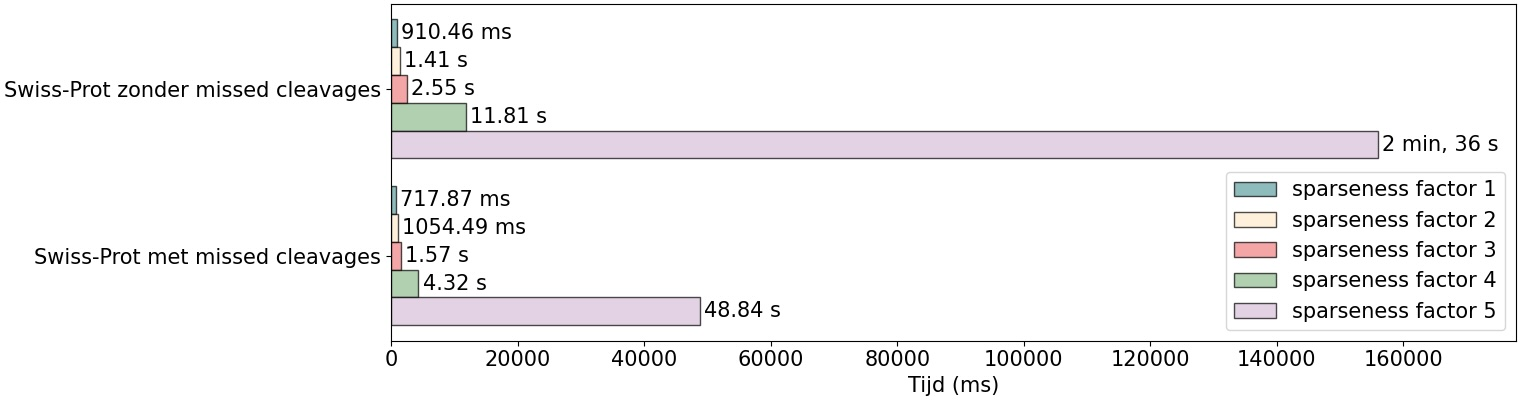
\includegraphics[width=\linewidth]{swissprot_searchtime_sparseness}}\\[4ex] % [4ex] om wat extra vertical spacing in te voegen

    \subfloat[Grootte van de volledige index en SSA voor de Swiss-Prot databank met sparseness factor $k = 1, 2, 3, 4, 5$.]{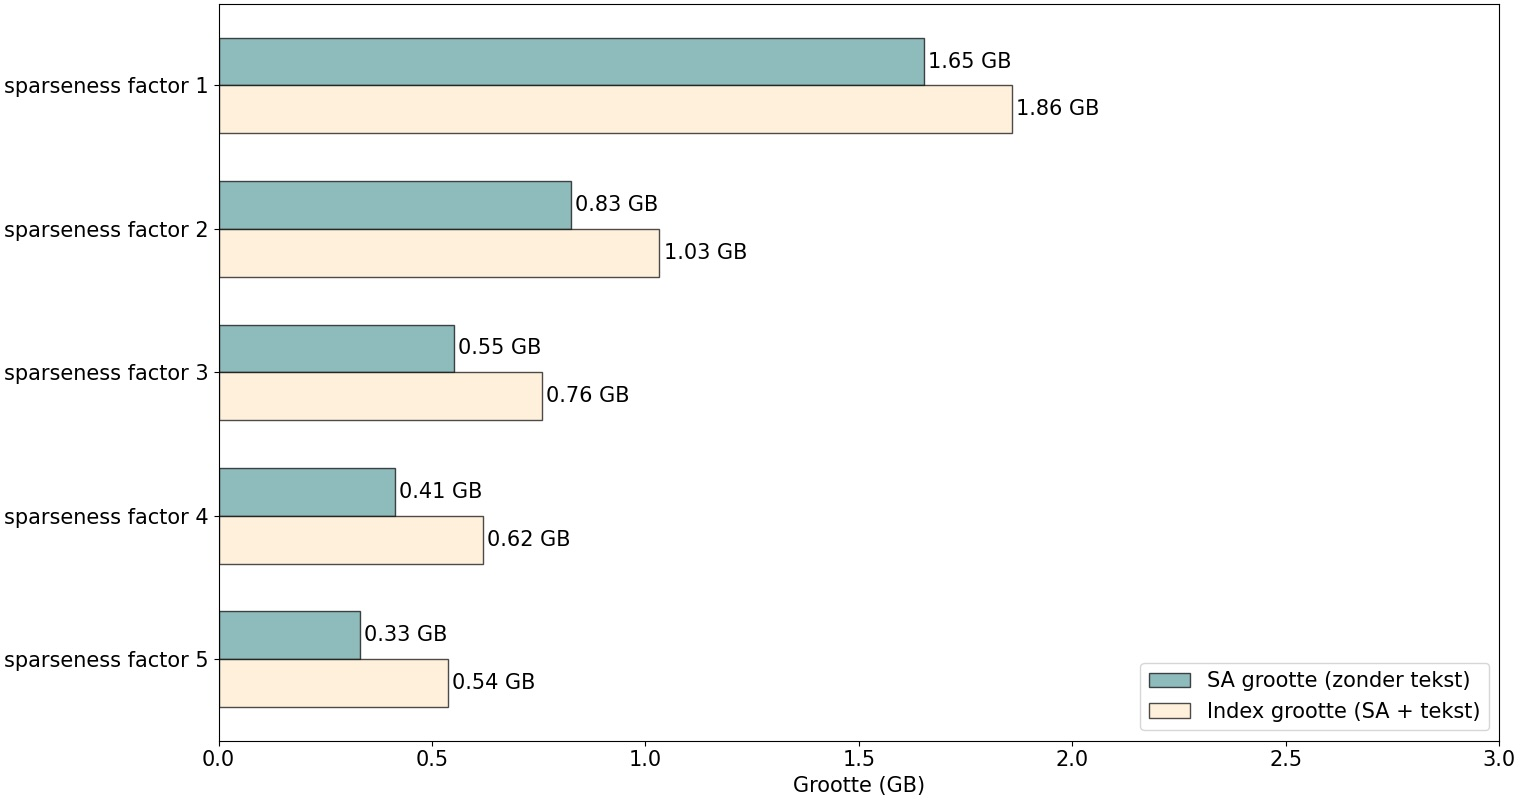
\includegraphics[width=0.8\linewidth]{index_size_SSA}}
    \caption{Zoektijd en indexgrootte van een SSA voor Swiss-Prot met $k = 1, 2, 3, 4, 5$.}\label{fig:search_sparseness}
\end{figure}

De zoektijd explodeert wanneer we de sparseness factor $k$ verhogen, omdat een deel van de gezochte peptiden bestaat uit 5 aminozuren.
Wanneer we deze proberen zoeken in een SSA met sparseness factor 5, zoeken we eigenlijk enkel één letter in de SSA (de laatste van de peptide).
Dit zal erg veel matches opleveren, en op zijn beurt erg veel werk vereisen om alle prefixen te controleren.
\\ \\
Anderzijds zal het verhogen van de sparseness factor de indexgrootte verkleinen.
Hierbij is het belangrijk dat enkel de SA mee verkleint.
Er blijft \textbf{altijd een vaste hoeveelheid geheugen nodig om de tekst zelf op te slaan}.
In Figuur~\ref{fig:search_sparseness}~(b) is duidelijk te zien dat, voor dit geval, de overgang van sparseness factor 4 naar 5 erg weinig winst heeft qua nodige opslagruimte, maar een grote impact heeft op de performantie.
\\ \\
Er zijn dus twee erg belangrijke bevindingen over sparse suffix arrays, en de manier waarop wij ze opbouwen.
\begin{enumerate}
    \item Probeer de sparseness factor zo laag mogelijk te houden, zo blijft ook de zoektijd voor kortere peptiden beperkt.
    \item Het maximale geheugengebruik voor het opbouwen van de SSA blijft constant onafhankelijk van de sparseness factor.
    De hoeveelheid geheugen om ze nadien te gebruiken kunnen we wel verkleinen.
    Hierdoor kan de index op minder krachtige machines gebruikt worden na het opbouwen.
\end{enumerate}

Dit impliceert dat we de sparseness factor $k$ enkel moeten verhogen om het geheugengebruik te beperken bij een al opgebouwde indexstructuur.
Dit is vooral van toepassing voor UniProtKB waar het nuttig is om kort een krachtige machine te gebruiken die de SA bouwt, waarna een minder krachtige machine de SSA host.
In het perfecte geval wordt \textbf{de sparseness factor zo gekozen zodat de SSA samen met de tekst net in het RAM geheugen past} van deze minder krachtige machine.


\section{Parallellisatie}\label{sec:parallellisatie}
Om het zoeken nog verder te versnellen, kan gebruikgemaakt worden van parallellisatie.
We hebben namelijk een \textbf{groot aantal peptiden} waarvoor we telkens dezelfde \textbf{statische indexstructuur} moeten doorzoeken.
Rust maakt dit proces vrij simpel omdat het \textit{ownership} systeem dataraces voorkomt (behalve wanneer gebruikgemaakt wordt van \textit{unsafe} code of het \textit{interior mutability} patroon)\cite{rust_data_races}.
Om een datatype te gebruiken in combinatie met multithreading moet deze de \texttt{Sync} en \texttt{Send} trait implementeren.
Deze traits worden door het typesysteem automatisch afgeleid.
Namelijk, wanneer alle componenten van een type aan de \texttt{Sync} en \texttt{Send} trait voldoen, dan voldoet je nieuwe type ook automatisch.
\\ \\
Uiteindelijk hebben we twee geparallelliseerde implementaties gemaakt.
In de eerste wordt alles volledig zelf beheerd.
Hierbij verdelen we zelf welke data naar welke thread gaat, worden de threads manueel opgestart en sluiten we ze ook zelf af.
In de tweede implementatie wordt gebruikgemaakt van de Rayon crate~\cite{rayon}.
Deze laat toe om op een simpele manier een sequentiële lus over een variabele te parallelliseren.
In ons geval was het omzetten van een sequentiële implementatie (nadat alle types voldeden aan de \texttt{Sync} en \texttt{Send} trait) zo simpel als het vervangen van \texttt{.iter()} door \texttt{.par\_iter()}.
Ook in deze implementatie is het mogelijk om manueel een specifiek aantal threads te kiezen.
Standaard gebruikt Rayon het aantal beschikbare logische cores op de machine, maar het instellen van een ander aantal kan aan de hand van één lijntje code.

\begin{minted}{Rust}
// Sequentieel
let results = peptiden
    .iter()
    .map(|peptide| search_peptide(peptide))
    .collect();

// Parallel
let results = peptiden
    .par_iter()
    .map(|peptide| search_peptide(peptide))
    .collect();
\end{minted}

\subsection{Manueel threaden vs Rayon}\label{subsec:manueel-threaden-vs-rayon}
Aangezien we twee verschillende implementaties hebben, is het interessant om na te gaan hoe deze ten opzichte van elkaar presteren.
Figuur~\ref{fig:threading_default_vs_rayon} toont de evolutie van de zoektijden voor een verschillend aantal threads.
We zien duidelijk dat de versie die gebruikmaakt van \textbf{Rayon net iets sneller} is en dat beide implementaties ongeveer \textbf{lineair schalen}.
De schaling is niet perfect één-op-één ten opzichte van het aantal threads omdat het inlezen en uitschrijven van de output sequentieel blijft.
Het verschil in uitvoeringstijd valt mogelijks te verklaren aan de manier waarop de data verdeeld wordt over de threads, in combinatie met een efficiëntere manier om de resultaten uit de threads te verwerken.
In de eigen implementatie kreeg elke thread simpelweg $\frac{1}{x}$ van alle peptiden toegekend, met $x$ het aantal threads.
De resultaten moeten daarna aan de hand van enkele stappen uit de thread-scope gehaald worden zodat deze terug beschikbaar zijn voor de rest van het programma.
Rayon maakt gebruik van een ingewikkelder systeem aan de hand van \textit{work stealing}~\cite{rayon_stealing} om de data over de threads te verdelen.

\begin{figure}[H]
    \centering
    \subfloat[Absolute uitvoeringstijd voor 1--12 threads.]{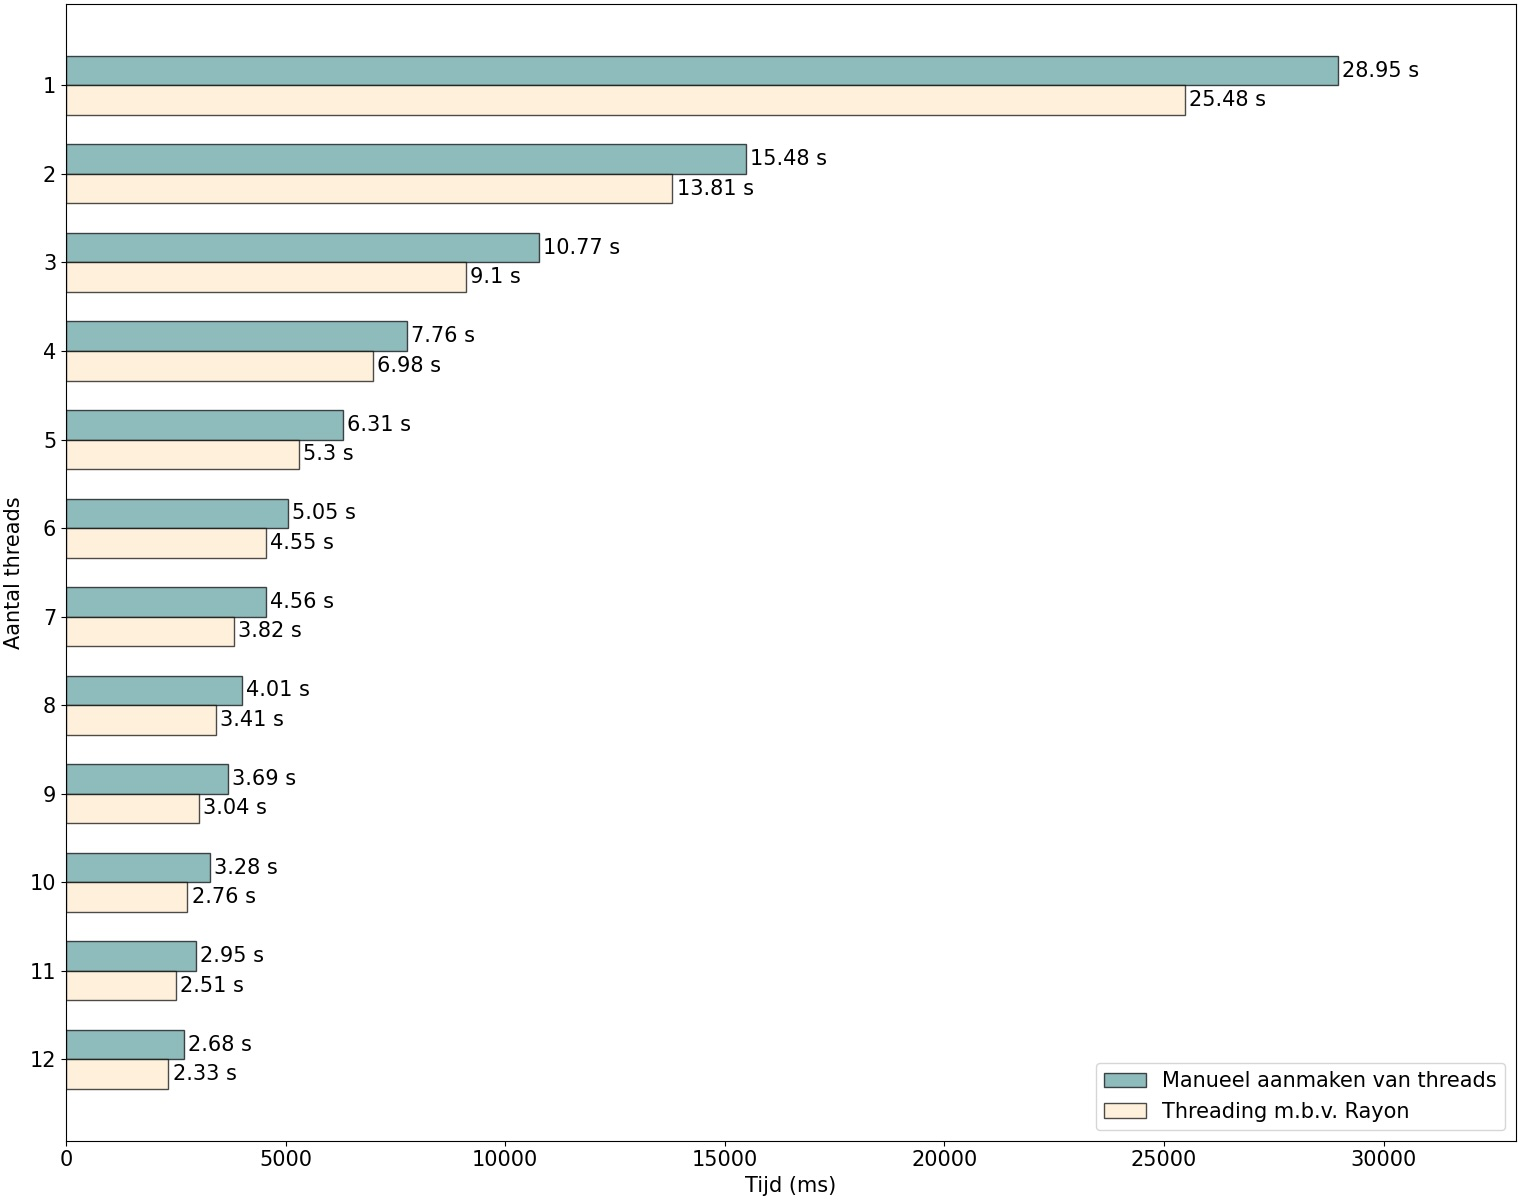
\includegraphics[width=0.7\linewidth]{threading_default_vs_rayon}}\\[4ex] % [4ex] om wat extra vertical spacing in te voegen

    \subfloat[Relatieve versnelling ten opzichte van uitvoering op 1 thread.]{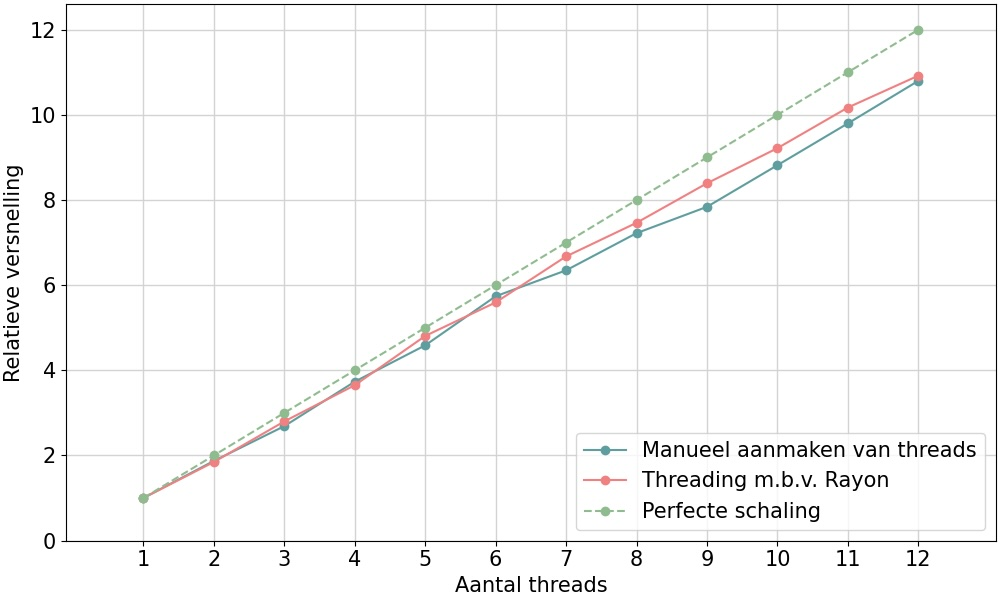
\includegraphics[width=0.7\linewidth]{threading_default_vs_rayon_relative}}
    \caption{Tijdsmeting om het Swiss-Prot peptidebestand zonder \textit{missed cleavages} te zoeken in een index met sparseness factor 3 voor 5\% van UniProtKB.}\label{fig:threading_default_vs_rayon}
\end{figure}

Naast het verschil in performantie zijn er nog andere voordelen verbonden aan het gebruik van Rayon.
De \textbf{code is namelijk veel simpeler en daarom ook beter te onderhouden}.
Dit motiveert onze keuze om finaal gebruik te maken van Rayon.


\section{Suffix arrays vs Suffixbomen}\label{sec:performantie}
Nu we verschillende manier verkend hebben om suffix arrays op te bouwen, is het interessant om suffix arrays te vergelijken met suffixbomen.
Op basis hiervan kunnen we vaststellen welke verbeteringen we gemaakt hebben, of deze indexstructuur goed genoeg schaalt om toepasbaar te zijn op de volledige UniProtKB databank en in welke tijd de peptiden gezocht kunnen worden.

\subsection{Opbouwen}\label{subsec:opbouwen}
Figuur~\ref{fig:array_building} visualiseert de tijd nodig om de indexstructuur op te bouwen in combinatie met het geheugengebruik.
Er is duidelijk een \textbf{mooie tijdswinst} verkregen, wat een bonus is voor het lokaal opbouwen van indices.
Voor het opbouwen van de index op UniProtKB is dit echter minder van belang aangezien dit proces slechts om de 8 weken moet gebeuren.
Zolang de nodige CPU-tijd hiervoor niet langer dan één à twee dagen is, is dit acceptabel.
Een veel belangrijkere vaststelling is het \textbf{maximale geheugengebruik tijdens opbouwen}.
Ook dit is \textbf{drastisch gedaald}.
Dit is exact de reden dat we deze indexstuctuur gekozen hebben.
Wanneer we het resultaat voor Swiss-Prot extrapoleren naar UniProtKB, gebruikmakende van de assumptie dat UniProtKB ongeveer 500 keer groter is, dan is de verwachting dat er ongeveer 1.2 TB RAM nodig zal zijn.
Hierbij heeft de sparseness factor $k$ geen invloed op het maximale geheugenverbruik tijdens het opbouwen van de suffix array.
We moeten namelijk eerst de volledige suffix array bouwen om daarna te samplen hieruit.
Deze 1.2 TB blijft een grote hoeveelheid aan geheugen, maar is wel al beschikbaar op de huidige generatie aan servers.
Zo bieden zowel Amazon via AWS, google via GCP en Microsoft via Azure instanties aan met enkele TB aan RAM\@.

\begin{figure}[H]
    \centering
    \subfloat[Tijd nodig om de indexstructuur op te bouwen.]{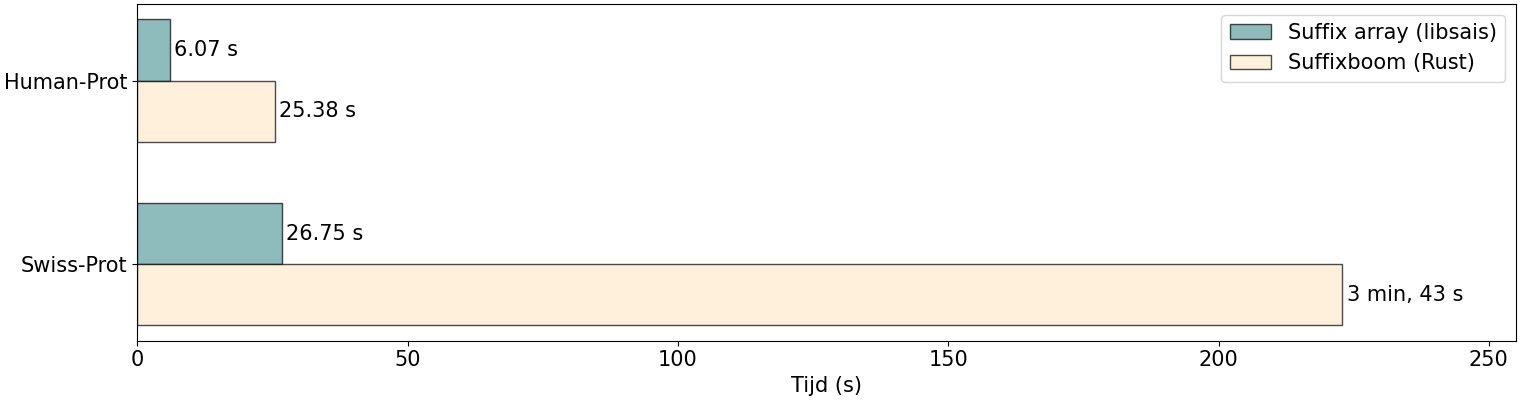
\includegraphics[width=\linewidth]{building_array_libsais_time}}\\[4ex] % [4ex] om wat extra vertical spacing in te voegen

    \subfloat[Maximaal geheugengebruik om de indexstructuur op te bouwen.]{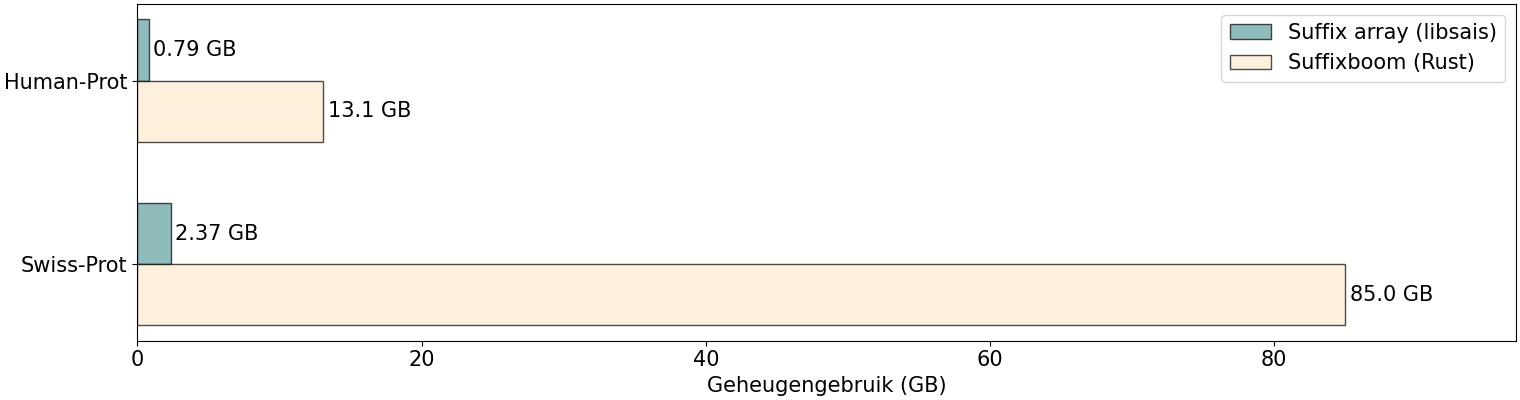
\includegraphics[width=\linewidth]{building_array_libsais_memory}}
    \caption{Vergelijking tussen de nodige tijd en hoeveelheid geheugen om een suffix array met libsais of een suffixboom in onze eigen Rust implementatie op te bouwen. De tijd en het geheugengebruik zijn gemeten met het Unix \texttt{time} commando. Als invoerbestand gebruiken we hier de Swiss-Prot of Human-Prot eiwitdatabank.}\label{fig:array_building}
\end{figure}

\subsection{Zoeken}\label{subsec:zoeken}
Aangezien er met de SA-indexstructuur geen voorberekening gebeurt van LCA's, is het enkel nuttig om de zoektijd inclusief het berekenen van de LCA te bekijken.
De tijd tot een match levert ons in dat geval nog niet alle nodige informatie op, zoals dit wel het geval was bij de suffixboom.
\\ \\
Figuur~\ref{fig:cutoff_humanprot}~(a) toont de zoekperformantie met suffix arrays.
Hier is onmiddellijk zichtbaar de de performantie voor het Human-Prot zoekbestand significant slechter is.
Na wat onderzoek bleek dat het berekenen van de LCA* erg traag werd indien er een groot aantal matches was.
Daarom is er besloten om een \textbf{drempelwaarde} (laten we deze B, van bovengrens, noemen) in te stellen.
Indien een peptide meer dan dan B matches heeft, wordt verondersteld dat de wortel de laagste gemeenschappelijke voorouder is van alle matches.
Uit eerder onderzoek uitgevoerd door het Unipept-team~\cite{unipept_cutoff} op de Unipept index die gebouwd was op basis van UniProt 2023\_03 bleek dat dit in de praktijk in de overgrote meerderheid van de gevallen ook effectief het geval is.
De resultaten hiervan kunnen teruggevonden worden in de tabellen in appendix~\ref{ch:appendix-unipept-protein-counts-distribution}.
Zo zijn er slechts $\pm$ 13\thinspace000 van de 1.3 miljard tryptische peptiden die meer dan 10\thinspace000 eiwitten matchen.
Hierbij was voor 95\% van de peptiden de LCA gelijk aan de wortel.
Slechts voor 200 peptiden was er een resultaat op soortniveau.
\\
\begin{figure}[H]
    \centering
    \subfloat[Bereken de LCA* voor alle matches. Voor de suffix arrays is gebruik gemaakt van sparseness factor $k = 1$.]{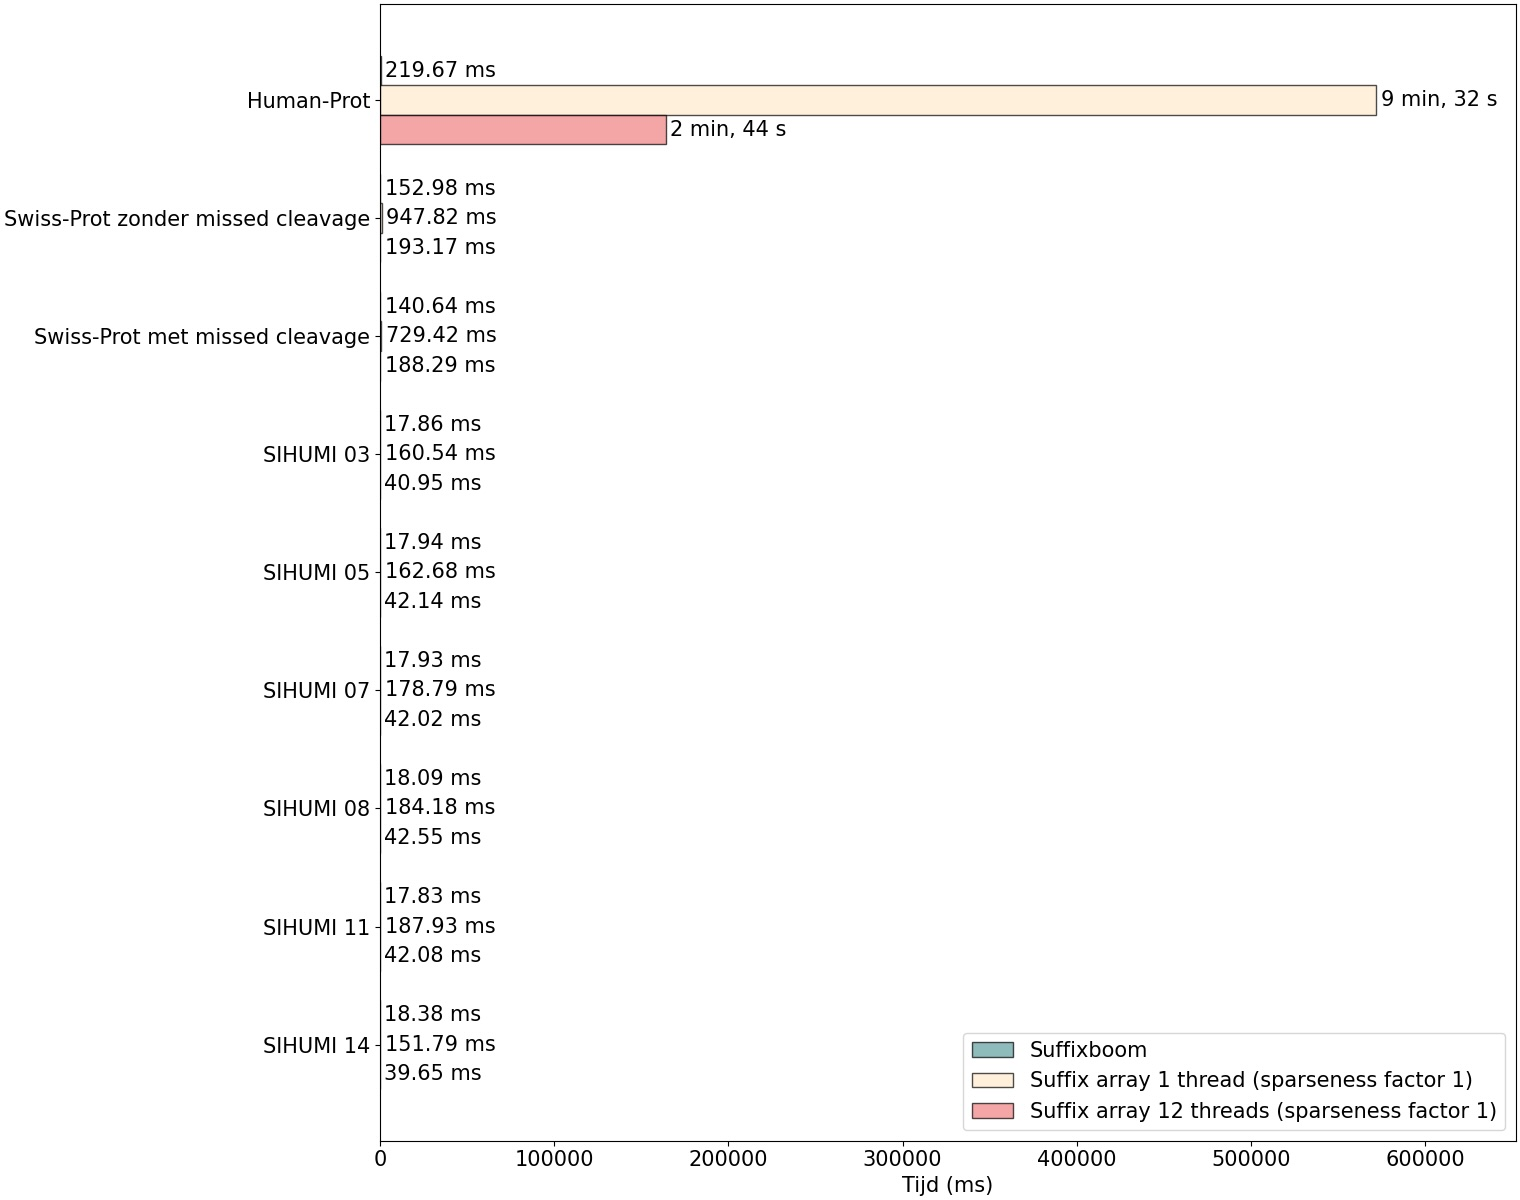
\includegraphics[width=0.7\linewidth]{no_cutoff_humanprot_search}}\\[4ex] % [4ex] om wat extra vertical spacing in te voegen

    \subfloat[Bereken de LCA* enkel als er minder dan 10\thinspace000 matches zijn.]{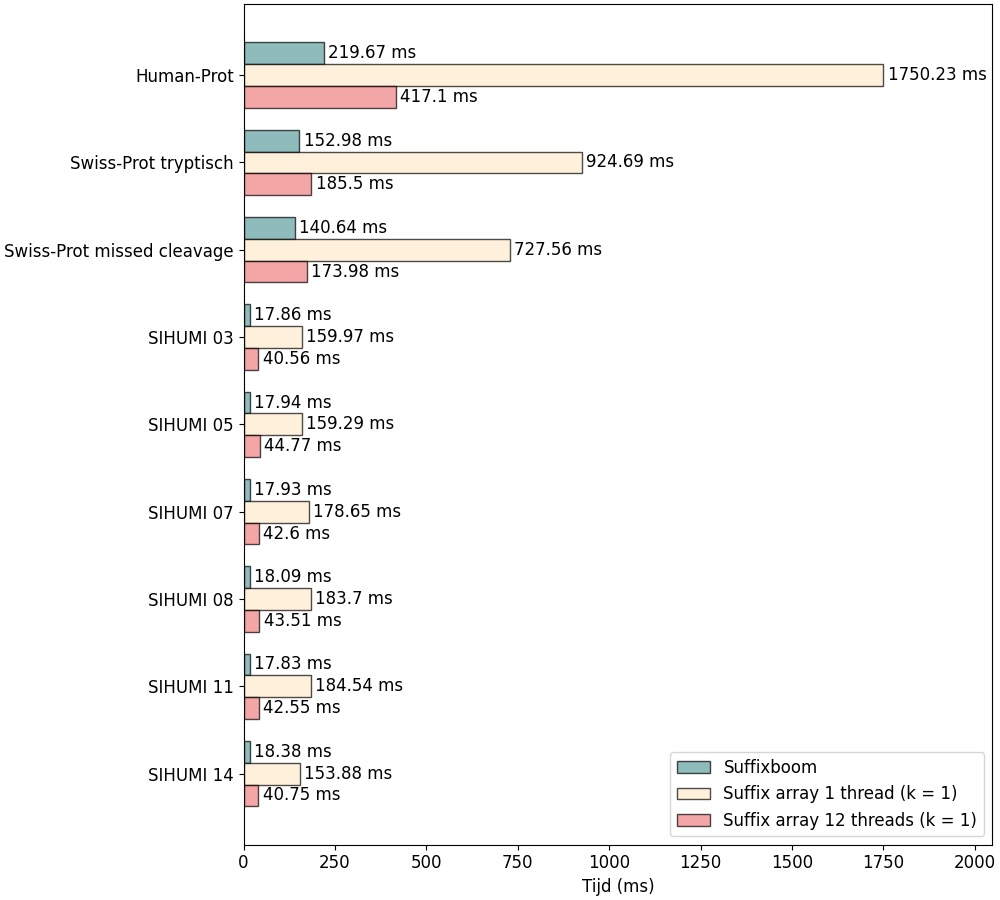
\includegraphics[width=0.7\linewidth]{cutoff_humanprot_search}}
    \caption{Berekenen van de LCA* (inclusief zoeken) voor alle peptiden (a) zonder en (b) met het gebruik van de drempelwaarde (B=10\thinspace000) op het Human-Prot en Swiss-Prot proteïnenbestand. De suffix array maakt gebruik van sparseness factor $k = 1$.}\label{fig:cutoff_humanprot}
\end{figure}

In Figuur~\ref{fig:cutoff_humanprot} is duidelijk te zien dat de \textbf{uitvoeringstijd drastisch daalt} wanneer de cut-off op 10000 matches geplaatst wordt.
Als we dit specifiek bekijken voor de Human-Prot peptidebestanden en eiwitdatabank is de uitvoeringstijd maar liefst 300 keer sneller.
Bovendien is ook hier het \textbf{informatieverlies minimaal}.
Van de 250\thinspace000 peptiden zijn er 12 peptiden die een ander resultaat verkrijgen in de output.
Deze 12 peptiden zijn echter slechts twee unieke peptiden (die gewoon meerdere keren voorkomen in het peptidebestand).
Dit zijn de peptiden \texttt{EKP} en \texttt{SKE}.
Indien we de LCA* effectief berekenen is het resultaat in beide gevallen 9606, terwijl we met een cut-off de root (1) terug geven.
\\ \\
Nu we het zoeken in de suffix array afgetopt hebben aan de hand van een cut-off, is het interessant om te kijken hoe de zoekperformantie zich verhoudt ten opzichte van het zoeken in een suffixboom.
In de praktijk is het zoeken in een suffix array 5 tot 10 maal trager voor onze testbestanden.
Een deel van deze extra zoektijd kan opgevangen worden door gebruik te maken van parallel zoeken.
Indien we hier gebruik van maken, duurt het zoeken van 100\thinspace000 peptiden op de Human-Prot en Swiss-Prot databank opnieuw enkele tientallen tot honderden milliseconden.
Natuurlijk zouden we het zoeken in een suffixboom ook kunnen parallelliseren, maar dit hebben we niet geprobeerd omwille van de eerder vermelde geheugenproblemen bij suffixbomen.

